%─────────────────%
% Header Settings %
%─────────────────%
\def\lecturer{SongHao}
\def\noter{THF}
\def\className{Probability Theory and Mathematical Statistics}
\def\term{III-A}
%─────────────────────%
% Undefined Variables %
%─────────────────────%
\ifx\noter\undefined
    \def\noter{THF}
\else
\fi
\ifx\lecturer\undefined
    \def\lecturer{None}
\else
\fi

%───────────────────%
% Document Settings %
%───────────────────%
\documentclass[12pt,a4paper]{article}

%─────────────────%
% Package Imports %
%─────────────────%
\usepackage[]{amsmath}
\usepackage[]{amssymb}
\usepackage[]{amsthm}
\usepackage[]{array}
\usepackage[]{bm}
\usepackage[]{booktabs}
\usepackage[UTF8]{ctex}
\usepackage[]{fancyhdr}
\usepackage[]{float}
\usepackage[]{geometry}
\usepackage[]{graphicx}
\usepackage[]{hyperref}
\usepackage[]{import}
\usepackage[]{inputenc}
\usepackage[]{mathrsfs}
\usepackage[]{multirow}
\usepackage[]{pdfpages}
\usepackage[]{pgfplots}
\usepackage[]{stmaryrd}
\usepackage[]{tabu}
\usepackage[]{tcolorbox}
\usepackage[]{textcomp}
\usepackage[]{thmtools}
\usepackage[]{tikz}
\usepackage[]{tkz-euclide}
\usepackage[]{url}
\usepackage[]{wrapfig}
\usepackage[dvipsnames]{xcolor}
\usepackage[]{xifthen}
\usepackage[]{yhmath}

%────────────────%
% Fancy Settings %
%────────────────%
\fancypagestyle{CustomStyle}{%
    \fancyhf{}
    \setlength{\headheight}{14.49998pt}
    \fancyhead[R]{\thepage}
    \fancyhead[L]{\lecturer: \className}
}

%──────────────────%
% pgfplot Settings %
%──────────────────%
\usepgfplotslibrary{external}
\pgfarrowsdeclarecombine{twolatex'}{twolatex'}{latex'}{latex'}{latex'}{latex'}
\pgfplotsset{compat=1.12}

%───────────────%
% Tikz Settings %
%───────────────%
\usetikzlibrary{arrows.meta}
\usetikzlibrary{decorations.markings}
\usetikzlibrary{decorations.pathmorphing}
\usetikzlibrary{positioning}
\usetikzlibrary{fadings}
\usetikzlibrary{intersections}
\usetikzlibrary{cd}
\tikzset{->/.style = {decoration={markings,mark=at position 1 with {\arrow[scale=2]{latex'}}},postaction={decorate}}}
\tikzset{<-/.style = {decoration={markings,mark=at position 0 with {\arrowreversed[scale=2]{latex'}}},postaction={decorate}}}
\tikzset{<->/.style = {decoration={markings,mark=at position 0 with {\arrowreversed[scale=2]{latex'}},mark=at position 1 with {\arrow[scale=2]{latex'}}},postaction={decorate}}}
\tikzset{->-/.style = {decoration={markings,mark=at position #1 with {\arrow[scale=2]{latex'}}},postaction={decorate}}}
\tikzset{-<-/.style = {decoration={markings,mark=at position #1 with {\arrowreversed[scale=2]{latex'}}},postaction={decorate}}}
\tikzset{->>/.style = {decoration={markings,mark=at position 1 with {\arrow[scale=2]{latex'}}}postaction={decorate}}}
\tikzset{<<-/.style = {decoration={markings,mark=at position 0 with {\arrowreversed[scale=2]{twolatex'}}},postaction={decorate}}}
\tikzset{<<->>/.style = {decoration={markings,mark=at position 0 with {\arrowreversed[scale=2]{twolatex'}},mark=at position 1 with {\arrow[scale=2]{twolatex'}}},postaction={decorate}}}
\tikzset{->>-/.style = {decoration={markings,mark=at position #1 with {\arrow[scale=2]{twolatex'}}},postaction={decorate}}}
\tikzset{-<<-/.style = {decoration={markings,mark=at position #1 with {\arrowreversed[scale=2]{twolatex'}}},postaction={decorate}}}
\tikzset{circ/.style = {fill, circle, inner sep = 0, minimum size = 3}}
\tikzset{scirc/.style = {fill, circle, inner sep = 0, minimum size = 1.5}}
\tikzset{mstate/.style={circle, draw, blue, text=black, minimum width=0.7cm}}
\tikzset{eqpic/.style={baseline={([yshift=-.5ex]current bounding box.center)}}}
\tikzset{commutative diagrams/.cd,cdmap/.style={/tikz/column 1/.append style={anchor=base east},/tikz/column 2/.append style={anchor=base west},row sep=tiny}}

%──────────────────────%
% Theorem Environments %
%──────────────────────%
\theoremstyle{definition}
\declaretheoremstyle[
    headfont=\bfseries\sffamily\color{ForestGreen!70!black}, bodyfont=\normalfont,
    mdframed={
        linewidth=2pt,
        rightline=false, topline=false, bottomline=false,
        linecolor=ForestGreen, backgroundcolor=ForestGreen!5,
    }
]{thmgreenbox}
\declaretheoremstyle[
    headfont=\bfseries\sffamily\color{NavyBlue!70!black}, bodyfont=\normalfont,
    mdframed={
        linewidth=2pt,
        rightline=false, topline=false, bottomline=false,
        linecolor=NavyBlue, backgroundcolor=NavyBlue!5,
    }
]{thmbluebox}
\declaretheoremstyle[
    headfont=\bfseries\sffamily\color{NavyBlue!70!black}, bodyfont=\normalfont,
    mdframed={
        linewidth=2pt,
        rightline=false, topline=false, bottomline=false,
        linecolor=NavyBlue
    }
]{thmblueline}
\declaretheoremstyle[
    headfont=\bfseries\sffamily\color{RawSienna!70!black}, bodyfont=\normalfont,
    mdframed={
        linewidth=2pt,
        rightline=false, topline=false, bottomline=false,
        linecolor=RawSienna, backgroundcolor=RawSienna!5,
    }
]{thmredbox}
\declaretheoremstyle[
    headfont=\bfseries\sffamily\color{RawSienna!70!black}, bodyfont=\normalfont,
    numbered=no,
    mdframed={
        linewidth=2pt,
        rightline=false, topline=false, bottomline=false,
        linecolor=RawSienna, backgroundcolor=RawSienna!1,
    },
    qed=\qedsymbol
]{thmproofbox}
\declaretheoremstyle[
    headfont=\bfseries\sffamily\color{NavyBlue!70!black}, bodyfont=\normalfont,
    numbered=no,
    mdframed={
        linewidth=2pt,
        rightline=false, topline=false, bottomline=false,
        linecolor=NavyBlue, backgroundcolor=NavyBlue!1,
    },
]{thmexplanationbox}
\declaretheorem[style=thmblueline,numbered=no,name=Notation]{notation}
\declaretheorem[style=thmgreenbox,numbered=no,name=Definition]{defi}
\declaretheorem[style=thmproofbox,numbered=no,name=Proof]{replacementproof}
\newtheorem*{aim}{Aim}
\newtheorem*{assumption}{Assumption}
\newtheorem*{axiom}{Axiom}
\newtheorem*{claim}{Claim}
\newtheorem*{conjecture}{Conjecture}
\newtheorem*{cor}{Corollary}
\newtheorem*{eg}{Example}
\newtheorem*{exercise}{Exercise}
\newtheorem*{ex}{Exercise}
\newtheorem*{fact}{Fact}
\newtheorem*{law}{Law}
\newtheorem*{lemma}{Lemma}
\newtheorem*{prop}{Proposition}
\newtheorem*{question}{Question}
\newtheorem*{remark}{Remark}
\newtheorem*{rrule}{Rule}
\newtheorem*{thm}{Theorem}
\newtheorem*{warning}{Warning}
% \newtheorem{ncor}[nthm]{Corollary}
% \newtheorem{nlemma}[nthm]{Lemma}
% \newtheorem{nprop}[nthm]{Proposition}
% \newtheorem{nthm}{Theorem}[section]
\renewenvironment{proof}[1][\proofname]{\vspace{-10pt}\begin{replacementproof}}{\end{replacementproof}}

%─────────────%
% Math Symbol %
%─────────────%

%────────────%
% Beginnings %
%────────────%
\title{\textbf{Part III-B: \className}}
\author{Lecture by \lecturer\\Note by \noter}
\pagestyle{CustomStyle}
%────────────────────────────────%
% Page Settings (set when print) %
%────────────────────────────────%
% \addtolength{\parskip}{-1mm}
% \addtolength{\parindent}{-2mm}
% \geometry{left=0.5cm,right=0.5cm,top=0.5cm,bottom=0.5cm}


%──────────%
% Document %
%──────────%
\begin{document}
\maketitle
\tableofcontents
\section{引言}%
\label{sec:引言}
\subsection{确定事件}%
\label{sub:确定事件}
一定发生的事件
\subsection{随机事件}
可能发生的事件
\subsection{统计规律}%
\label{sub:统计规律}
大量试验得出的宏观规律
\section{事件}%
\label{sec:事件}
\subsection{试验}%
\label{sub:试验}
对对象观察、测量、实验
\subsection{随机试验}%
\label{sub:随机试验}
随机试验的条件:\\
1. 在相同条件下可重复\\
2. 结果不止一个\\
3. 试验前无法预测出现的实验结果

使用$E$代表随机试验。
\subsection{事件}%
\label{sub:事件}
随机试验的每种结果。
\subsection{随机事件}%
\label{sub:随机事件}
可能出现的事件,用$A$,$B$,$C\dots$表示
\subsection{基本事件}%
\label{sub:基本事件}
不能或不必再分的事件(基于试验的事件)
\begin{eg}
	扔一次骰子,实验目的为:骰子朝上的点数,\\
	基本事件为:出现$1,2,3,4,5,6$点。
\end{eg}
\begin{eg}
	扔一次骰子,实验目的为:骰子的位置,\\
	此时出现的点数不是基本事件。
\end{eg}
\begin{eg}
	扔一次硬币,实验目的为:硬币朝上的面,\\
	基本事件为:出现正面或反面。
\end{eg}
\begin{eg}
	扔一次硬币,实验目的为:硬币某根已知的轴线与已知直线的夹角\\
	基本事件为:夹角$\theta\in [0,2\pi]$\\
	此时正面朝上与反面朝上不是基本事件。
\end{eg}
\subsection{复合事件}%
\label{sub:复合事件}
由基本事件复合而成的事件
\begin{eg}
	扔一次骰子,点数小于$7$点表示为:
	$$
	\Omega=\{x|x<7\}
	$$
	点数大于$7$点表示为:
	$$
	\varnothing=\{x|x>7\}
	$$
\end{eg}
\subsection{必然事件}%
\label{sub:必然事件}
一定发生的结果,用$\Omega$表示
\subsection{不可能事件}%
\label{sub:不可能事件}
不可能发生的结果,用$\varnothing$表示
\begin{eg}
	扔一次骰子,点数大于$7$点为不可能事件
\end{eg}
\subsection{样本空间}%
\label{sub:样本空间}
所有基本事件的集合(实验目的确定),与必然事件相似,用$\Omega$表示。
\subsection{样本点}%
\label{sub:样本点}
样本空间中的元素,即基本事件,用$\omega$表示。
\begin{eg}
	扔硬币研究某面朝上的样本空间:$\Omega=\{\mbox{正,反}\}$\\
	样本点:$\omega_1=\mbox{正面朝上}$,$\omega_2=\mbox{反面朝上}$
\end{eg}
\begin{eg}
	扔一个骰子研究某点朝上的样本空间:
	$$
	\Omega=\{x|x\in[1,6],x\in\mathbb{R}\}
	$$
	样本点:
	$$
	(\omega_1,\omega_2,\dots\omega_6) = (1,2,3,4,5,6)
	$$
\end{eg}
\begin{eg}
	扔两个硬币,研究朝上的面,样本空间为:
	$$
		\Omega=\{(x,y)|(0,0),(1,1),(0,1),(1,0))\}
	$$
	或:
	$$
		\Omega=\{(x,y)|x,y\in\{0,1\}\}
	$$
\end{eg}
\begin{notation}
	样本空间可以是无限集。
\end{notation}
\begin{eg}
	在$[0,1]$内扔一个质子,求其坐标。\\
	其样本空间为:
	$$
    \Omega=\{x|x\in[0,1]\}
	$$
\end{eg}
\begin{notation}
    质子/点:无大小
\end{notation}
\begin{eg}
	向平面扔一个点:
	$$
		\Omega=\{(x,y)|x,y\in\mathbb{R}\}
	$$
\end{eg}
\section{事件的集合表示}%
\label{sec:事件的集合表示}
集合(set):$A=\{2,4,6\}$等。
\begin{notation}
	$\Omega$与必然事件、样本空间等同,$\varnothing$与不可能事件、空集等同。\\
	任何事件都是$\Omega$的子集,$\varnothing$是所有事件的子集。
\end{notation}

\section{事件间的关系}
\subsection{包含}%
\label{sub:包含}
\begin{center}
	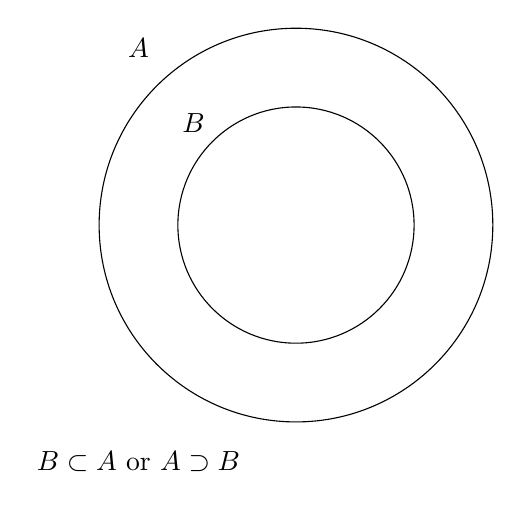
\begin{tikzpicture}
        \draw circle [radius=2.5];
		\draw circle [radius=1.5];
		\draw (-2,2) node [above] {$A$};
		\draw (-1.3,1.3) node {$B$};
		\draw (-2,-3) node {$B\subset A$ or $A\supset B$};
	\end{tikzpicture}
\end{center}
$A$发生必然有$B$发生,且有:
\[
\forall A,\varnothing\subset A\subset \Omega
.\] 
\subsection{相等}%
\label{sub:相等}
\begin{center}
    \begin{tikzpicture}
        \draw circle [radius=2];
        \draw (4,1) node {$B\subset A$ and $A\subset B$};
    \end{tikzpicture}
\end{center}
称$A$与$B$相等。
\subsection{并与和}%
\label{sub:并与和}
\begin{center}
    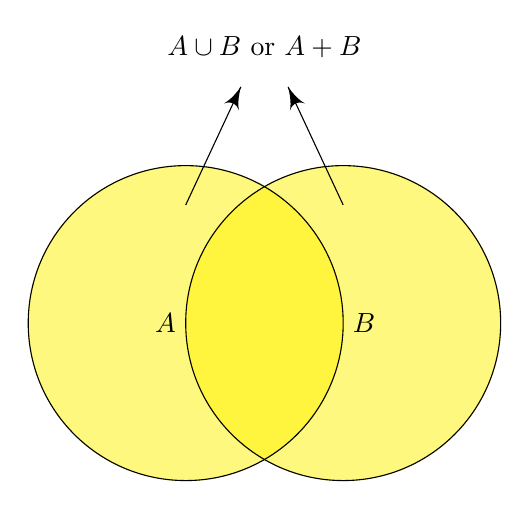
\begin{tikzpicture}
        \filldraw [yellow,opacity=0.5] (-1,0) circle [radius=2];
        \filldraw [yellow,opacity=0.5] (1,0) circle [radius=2];
        \draw (-1,0) circle [radius=2] node [left] {$A$};
        \draw (1,0) circle [radius=2] node [right] {$B$};
        \draw [->] (-1,1.5)--(-0.3,3);
        \draw [->] (1,1.5)--(0.3,3);
        \draw (0,3.5) node {$A\cup B$ or $A+B$};
    \end{tikzpicture}
\end{center}
$A\cup B:$(并/和)$A$与$B$至少有一个发生
$$
\begin{cases}
    &A+B\subset A,\\
    &A+A=A,\\
    &A+\varnothing=A,\\
    &A+\Omega=\Omega.
\end{cases}
$$
\subsection{交与积}%
\label{sub:交与积}
\begin{center}
    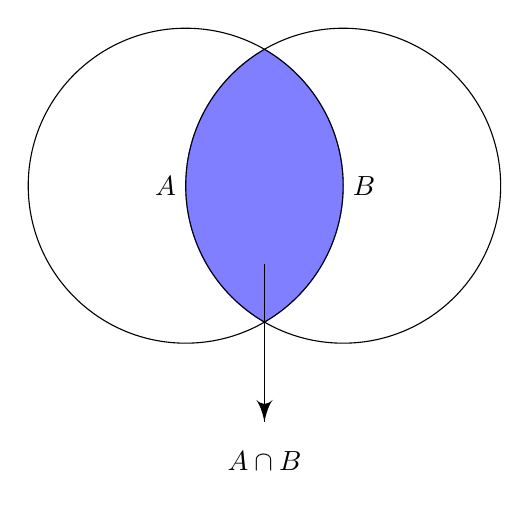
\begin{tikzpicture}
        \filldraw [blue,opacity=0.5] (0,1.732) arc (120:240:2) (0,-1.732) arc (-60:60:2);
        \draw (-1,0) circle [radius=2] node [left] {$A$};
        \draw (1,0) circle [radius=2] node [right] {$B$};
        \draw [->] (0,-1)--(0,-3) node at(0,-3.5) {$A\cap B$ };
    \end{tikzpicture}
\end{center}
$A\cap B:$(交/积)$A$与$B$同时发生
\begin{center}
    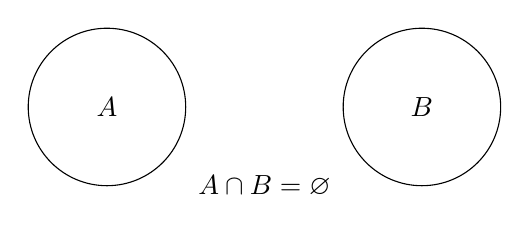
\begin{tikzpicture}
        \draw (-2,0) circle [radius=1] node {$A$};
        \draw (2,0) circle [radius=1] node {$B$};
        \draw (0,-1) node {$A\cap B=\varnothing $};
    \end{tikzpicture}
\end{center}
\begin{center}
    \begin{tikzpicture}
        \draw circle [radius=2] node at(-2,2) {$A$};
        \draw circle [radius=1] node at(-1,1) {$B$};
        \draw (4,0) node {$A\cap B=B$};
    \end{tikzpicture}
\end{center}
\[
    \begin{cases}
        AB\subset A\\
        AA=A\\
        A\varnothing=\varnothing\\
        A\Omega=A
    \end{cases}
.\]
\begin{defi}[]
    无限可列个:能按某种规律排成一个序列
\end{defi}
\begin{eg}[]
    自然数无限可列:$0,1,2,\ldots$
\end{eg}
\begin{eg}[]
    整数无限可列:$0,1,-1,2,-2,\ldots$
\end{eg}
\begin{eg}[]
    有理数:能写成$\displaystyle{\frac{p}{q}}$的数\\
    $0.\dot{5}\dot{6}$可以写为:$\displaystyle{\frac{56}{99}}$\\
    $0.1\dot{2}$可以写为:$\displaystyle{\frac{11}{90}}$\\
    有理数无限可列:$\displaystyle{0,\frac{1}{1},\frac{-1}{1},\frac{1}{2},\frac{-1}{2}\ldots}$
\end{eg}
\begin{eg}[]
    实数集、平面点集非无限可列。
\end{eg}
以下定义:
\begin{defi}
    $n$个事件互斥时:
    \[
         A_1\cup A_2\cup \ldots\cup A_{n}=\bigcup_{i=1}^{n}A_{i} \\
    .\]
    $n$个事件同时发生:
    \[
        A_1\cap A_2\cap \ldots\cap A_n=\bigcap_{i=1}^{n}A_{i}
    .\]
    该定义支持无限可列个。
\end{defi}
\subsection{差}
$A-B$:  $A$发生而 $B$ 不发生。
\begin{center}
    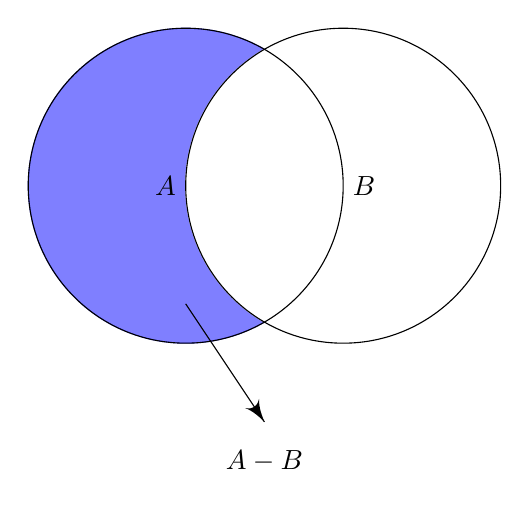
\begin{tikzpicture}
        \filldraw [blue,opacity=0.5] (-1,0) circle [radius=2];
        \filldraw [white] (1,0) circle [radius=2];
        \draw (1,0) circle [radius=2] node [right] {$B$};
        \draw (-1,0) circle [radius=2] node [left] {$A$};
        \draw [->] (-1, -1.5)--(0,-3) node at(0,-3.5) {$A-B$};
    \end{tikzpicture}
\end{center}
\begin{center}
    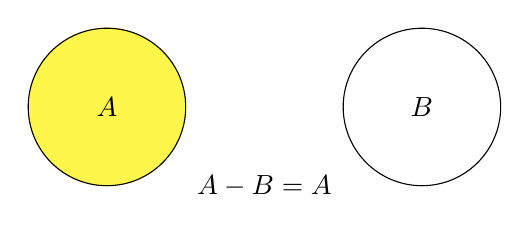
\begin{tikzpicture}
        \filldraw [yellow,opacity=0.7] (-2,0) circle [radius=1];
        \draw (-2,0) circle [radius=1] node {$A$};
        \draw (2,0) circle [radius=1] node {$B$};
        \draw (0,-1) node {$A-B=A$ };
    \end{tikzpicture}
\end{center}
\begin{center}
    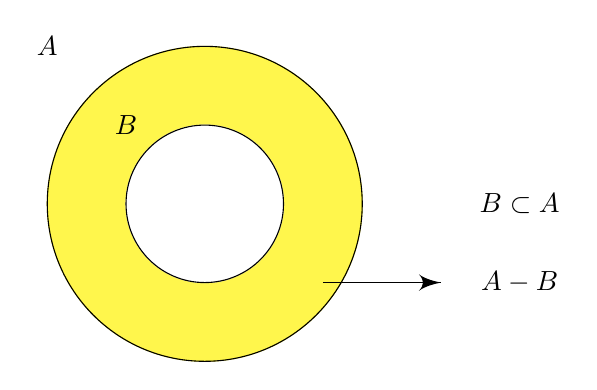
\begin{tikzpicture}
        \filldraw [yellow,opacity=0.7] circle [radius=2];
        \filldraw [white] circle [radius=1];
        \draw circle [radius=2] (-2,2) node {$A$ } (0,0) circle [radius=1] (-1,1) node {$B$ };
        \draw (4,0) node {$B\subset A$ };
        \draw [->] (1.5,-1)--(3,-1) node at(4,-1) {$A-B$ };
    \end{tikzpicture}
\end{center}
\begin{center}
    \begin{tikzpicture}
        \draw circle [radius=2] (-2,2) node {$B$ } (0,0) circle [radius=1] (-1,1) node {$A$ };
        \node[red] (AsubsetB) at (4,0) {$A\subset B$};
        \draw node at(4,-1) {$A-B=\varnothing$ };
    \end{tikzpicture}
\end{center}
\subsection{互不相容}%
\label{sub:互不相容}
$A$ 与$B $不同时发生,即:$AB=\varnothing$ 
\begin{center}
    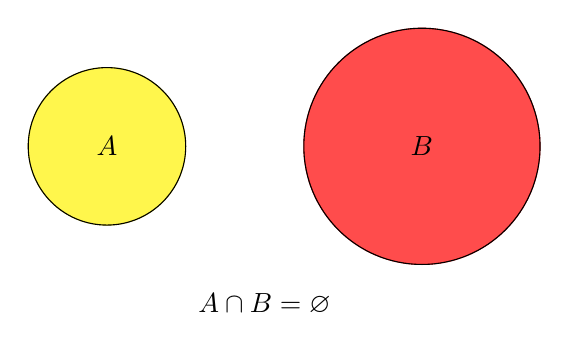
\begin{tikzpicture}
        \filldraw [yellow,opacity=0.7] (-2,0) circle [radius=1];
        \filldraw [red,opacity=0.7] (2,0) circle [radius=1.5];
        \node[] (A) at (-2,0) {$A$};
        \node[] (B) at (2,0) {$B$};
        \draw (-2,0) circle [radius=1];
        \draw (2,0) circle [radius=1.5];
        \node[] (AcapBvarnothing) at (0,-2) {$A\cap B=\varnothing$};
    \end{tikzpicture}
\end{center}
$n$ 个事件:
\[
    A_1,A_2,\ldots A_n
.\] 
互不相容,则:
\[
    \forall i,j: A_iA_j=\varnothing
.\] 
\subsection{对立}%
\label{sub:对立}
$AB=\varnothing$ 且$A\cup B=\Omega$ 
\begin{center}
    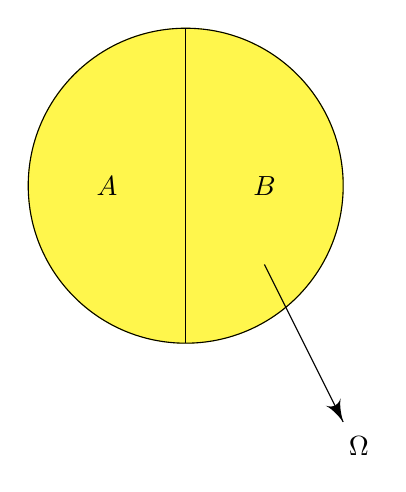
\begin{tikzpicture}
        \filldraw [yellow,opacity=0.7] circle [radius=2];
        \draw circle [radius=2];
        \draw (0,2)--(0,-2);
        \node[] (A) at (-1,0) {$A$};
        \node[] (B) at (1,0) {$B$};
        \draw [->] (1,-1)--(2,-3) node [] at(2.2,-3.3) {$\Omega$ };
    \end{tikzpicture}
\end{center}
记作: \[
    A=\overline{B}
.\] 
或:\[
    B=\overline{A}
.\]
由此可得:
\[
\begin{cases}
    \overline{\overline{A}}=A\\
    A-B=A-AB=A\overline{B}
\end{cases}
.\]
\begin{center}
    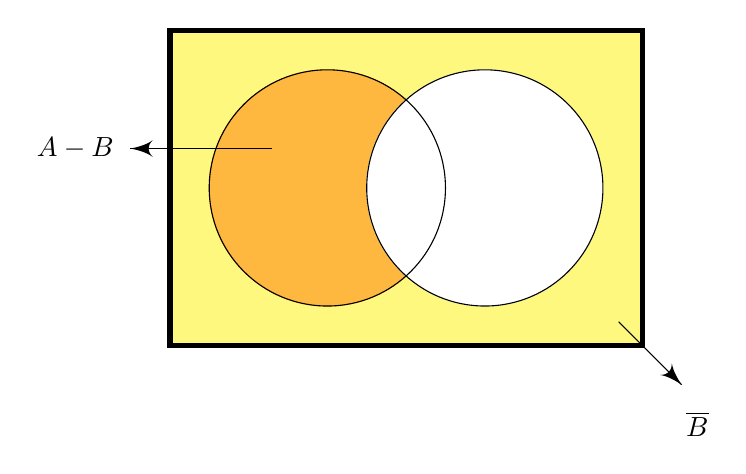
\begin{tikzpicture}
        \filldraw [red,opacity=0.5] (-1,0) circle [radius=1.5];
        \filldraw [yellow,opacity=0.5] (-3,2) rectangle (3,-2);
        \filldraw [white] (1,0) circle [radius=1.5];
        \draw [line width=2] (-3,2) rectangle (3,-2);
        \draw (-1,0) circle [radius=1.5] (1,0) circle [radius=1.5];
        \draw [->] (2.7,-1.7)--(3.5,-2.5) node at(3.7,-3) {$\overline{B}$ };
        \draw [->] (-1.7,0.5)--(-3.5,0.5) node at(-4.2,0.5) {$A-B$};
    \end{tikzpicture}
\end{center}
\begin{notation}
    若两事件对立,则一定互不相容.\\
    互不相容的事件不一定对立.
\end{notation}
\begin{notation}
    互不相容适用于多个事件.\\
    对立只适用于两个事件.
\end{notation}
\begin{center}
    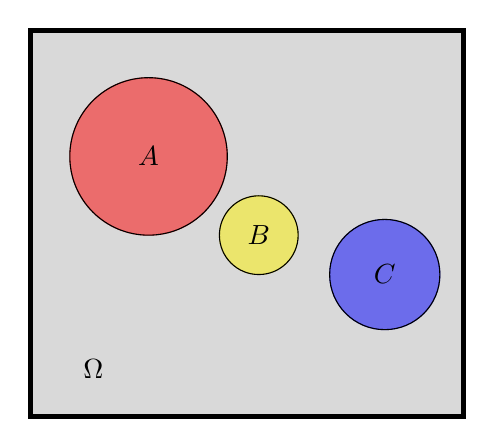
\begin{tikzpicture}
        \filldraw [gray,opacity=0.3] (-3.5,2.6) rectangle (2,-2.3);
        \filldraw [red,opacity=0.5] (-2,1) circle [radius=1];
        \filldraw [yellow,opacity=0.5] (-0.6,0) circle [radius=0.5];
        \filldraw [blue,opacity=0.5] (1,-0.5) circle [radius=0.7];
        \draw (-2,1) circle [radius=1] node {$A$ };
        \draw (-0.6,0) circle [radius=0.5] node {$B$ };
        \draw (1,-0.5) circle [radius=0.7] node {$C$ };
        \draw [line width=2] (-3.5,2.6) rectangle (2,-2.3) node at(-2.7,-1.7) {$\Omega$ };
    \end{tikzpicture}
\end{center}
\begin{notation}
    互不相容:不能同时发生,但可以都不发生\\
    对立:必须有一个发生
\end{notation}
\subsection{完备事件组}%
\label{sub:完备事件组}
$A_1,A_2,\ldots A_n$ 两两互不相容,且\[
    \bigcup_{i=1}^n A_i=\Omega
.\] 
则为完备事件组。
\begin{center}
    \begin{tikzpicture}
        \draw (-6,2) rectangle (6,-2);
        \draw (-5,2)--(-5,-2);
        \draw (-4,2)--(-4,-2);
        \draw (-3,2)--(-3,-2);
        \draw (-2,2)--(-2,-2);
        \draw (2,2)--(2,-2);
        \draw (3,2)--(3,-2);
        \draw (4,2)--(4,-2);
        \draw (5,2)--(5,-2);
        \node[] (A1) at(-5.5,0) {$A_1$};
        \node[] (A2) at (-4.5,0) {$A_2$};
        \node[] (A3) at (-3.5,0) {$A_3$};
        \node[] (A4) at (-2.5,0) {$A_4$};
        \node[] (ldots) at (0,0) {$\ldots$};
        \node[] (An1) at (4.5,0) {$A_{n-1}$};
        \node[] (An) at (5.5,0) {$A_n$};
        \draw [->] (6,-2)--(7,-3) node at (7,-3.5) {$\Omega$ };
    \end{tikzpicture}
\end{center}
\section{事件间的运算律}%
\label{sec:事件间的运算律}
\subsection{交换律}%
\label{sub:交换律}
\[
    \begin{cases}
        A\cup B=B\cup A\\
        A\cap B=B\cap A
    \end{cases}
.\] 
\subsection{结合律}%
\label{sub:结合律}
\[
    \begin{cases}
        (A\cup B)\cup C=A\cup (B\cup C)\\
        (A\cap B)\cap C=A\cap (B\cap C)
        
    \end{cases}
.\] 
\subsection{分配律}%
\label{sub:分配律}
\[
    (A\cup B)\cap C=(A\cap C)\cup (B\cap C)
.\] 
\begin{center}
    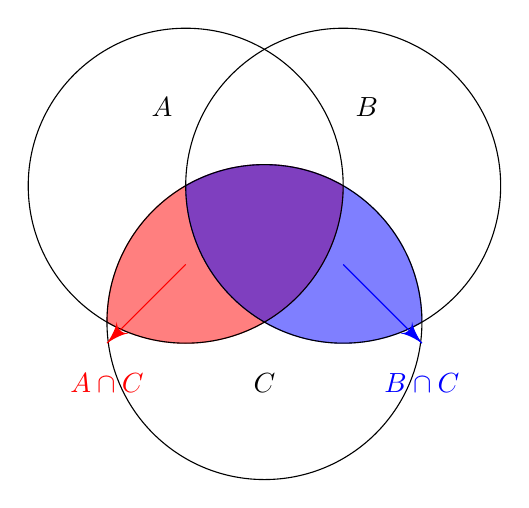
\begin{tikzpicture}
        \filldraw [red,opacity=0.5] (1,0) arc (60:180:2) (-2,-1.732) arc (240:360:2);
        \filldraw [blue,opacity=0.5] (-1,0) arc (180:300:2) (2,-1.732) arc (0:120:2);
        \draw (-1,0) circle [radius=2] node at(-1.3,1) {$A$ };
        \draw (1,0) circle [radius=2] node at (1.3,1) {$B$ };
        \draw (0,-1.732) circle [radius=2] node at (0,-2.5) {$C$ };
        \draw [->,red] (-1,-1)--(-2,-2) node [red] at(-2,-2.5) {$A\cap C$ };
        \draw [->,blue] (1,-1)--(2,-2) node [blue] at(2,-2.5) {$B\cap C$ };
    \end{tikzpicture}
\end{center}
\[
    (A\cap B)\cup C=(A\cup C)\cap (B\cup C)
.\] 
\begin{center}
    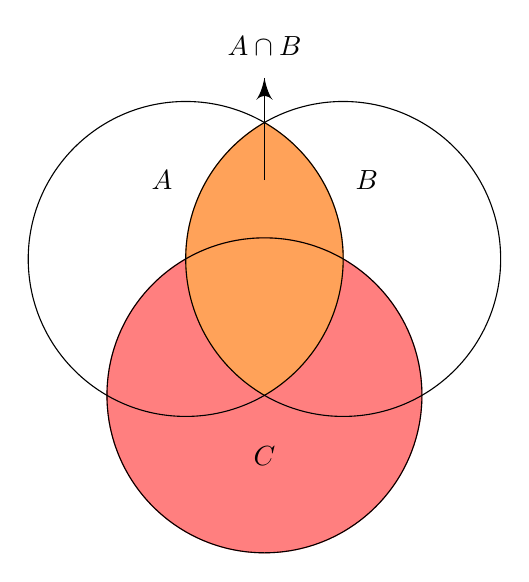
\begin{tikzpicture}
        \filldraw [red,opacity=0.5] (0,-1.732) circle [radius=2] (0,1.732) arc (120:240:2) (0,-1.732) arc (-60:60:2);
        \filldraw [yellow,opacity=0.3] (0,1.732) arc (120:240:2) (0,-1.732) arc (-60:60:2);
        \draw (-1,0) circle [radius=2] node at(-1.3,1) {$A$ };
        \draw (1,0) circle [radius=2] node at (1.3,1) {$B$ };
        \draw (0,-1.732) circle [radius=2] node at (0,-2.5) {$C$ };
        \draw [->] (0,1)--(0,2.3) node at(0,2.7) {$A\cap B$ };
    \end{tikzpicture}
\end{center}
\subsection{对偶律}%
\label{sub:对偶律}
\[
    \overline{A\cup B}=\overline{A}\cap \overline{B}
.\] 
\begin{center}
    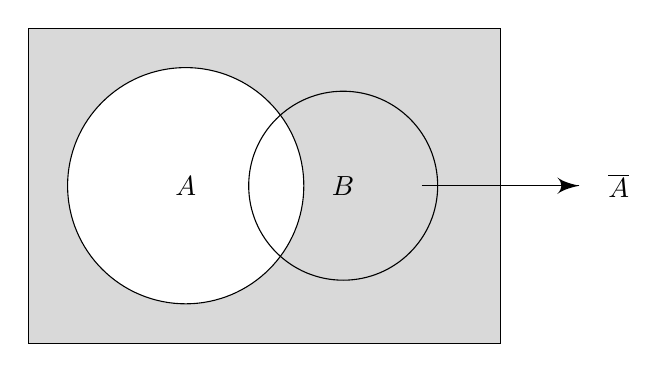
\begin{tikzpicture}
        \filldraw [gray,opacity=0.3] (-3,2) rectangle (3,-2); 
        \filldraw [white] (-1,0) circle [radius=1.5];
        \draw (-3,2) rectangle (3,-2);        
        \draw (-1,0) circle [radius=1.5] node {$A$ };
        \draw (1,0) circle [radius=1.2] node {$B$ };
        \draw [->] (2,0)--(4,0) node at(4.5,0) {$\overline{A}$ };
    \end{tikzpicture}
\end{center}
\begin{center}
    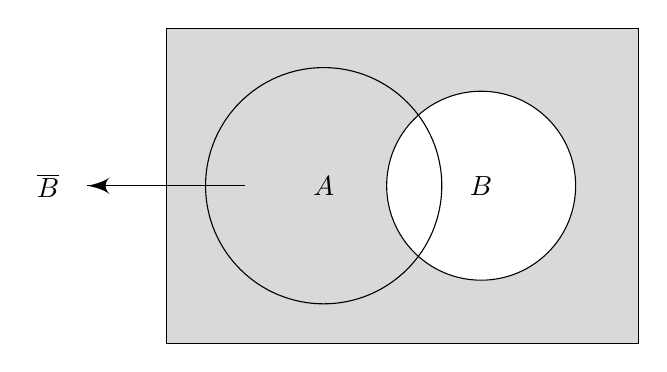
\begin{tikzpicture}
        \filldraw [gray,opacity=0.3] (-3,2) rectangle (3,-2); 
        \filldraw [white] (1,0) circle [radius=1.2];
        \draw (-3,2) rectangle (3,-2);        
        \draw (-1,0) circle [radius=1.5] node {$A$ };
        \draw (1,0) circle [radius=1.2] node {$B$ };
        \draw [->] (-2,0)--(-4,0) node at(-4.5,0) {$\overline{B}$ };
    \end{tikzpicture}
\end{center}
\begin{center}
    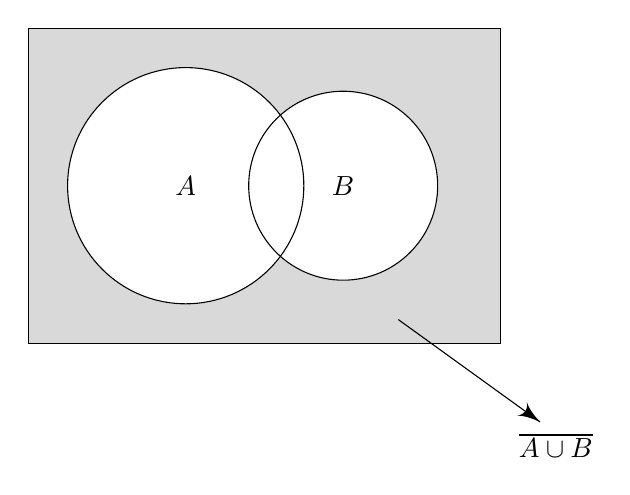
\begin{tikzpicture}
        \filldraw [gray,opacity=0.3] (-3,2) rectangle (3,-2); 
        \filldraw [white] (-1,0) circle [radius=1.5] (1,0) circle [radius=1.2];
        \draw (-3,2) rectangle (3,-2);        
        \draw (-1,0) circle [radius=1.5] node {$A$ };
        \draw (1,0) circle [radius=1.2] node {$B$ };
        \draw [->] (1.7,-1.7)--(3.5,-3) node at(3.7,-3.3) {$\overline{A\cup B}$ };
    \end{tikzpicture}
\end{center}
\[
    \overline{A\cap B}=\overline{A}\cup \overline{B}
.\] 
记法:

1. 画图

2. 长线变短线,开口换方向

3. 事件定义

\begin{notation}
    多个事件的对偶律:
    \[
        \begin{cases}
            \displaystyle{\overline{\bigcup_{i=1}^n A_i}=\bigcap_{i=1}^n \overline{A_i}}\\
            \displaystyle{\overline{\bigcap_{i=1}^n A_i}=\bigcup_{i=1}^{n} \overline{A_i}}
        \end{cases}
    .\] 
\end{notation}
\begin{eg}[]
    $A,B,C$ 是试验$E$ 的随机事件,用符号表示以下事件:
    
    1. 只有$A$ 发生:$A\bar{B}\bar{C}$

    2. $A$ 发生:A

    3. $A,B,C$ 只有一个发生:$A\bar{B}\bar{C}+\bar{A}B\bar{C}+\bar{A}\bar{B}C$

    4. $A,B,C$ 同时发生:$ABC$ 

    5. $A,B,C$ 至少一个发生:$A+B+C$ 

    6. $A,B,C$ 至多一个发生:$\bar{A}\bar{B}\bar{C}+A\bar{B}\bar{C}+\bar{A}B\bar{C}+\bar{A}\bar{B}C$

    7. $A,B,C$ 恰有两个发生:$AB\bar{C}+A\bar{B}C+\bar{A}BC$

    8. $A,B,C$ 至少两个发生:$AB\bar{C}+A\bar{B}C+\bar{A}BC+ABC$或$AB+BC+AC$
\end{eg}
\begin{eg}[]
    从产品中抽查,不放回,一共取了三次:$A_1,A_2,A_3$ 代表三次取得合格品:

    1. 三次都合格:$A_1A_2A_3$ 
    
    2. 至少一次合格:$A_1+A_2+A_3$ 

    3. 恰有两次合格:$A_1A_2\bar{A_3}+A_1\bar{A_2}A_3+\bar{A_1}A_2A_3$

    4. 最多一次合格:$\bar{A_1}\bar{A_2}\bar{A_3}+A_1 \bar{A_2}\bar{A_3}+\bar{A_1}A_2 \bar{A_3}+\bar{A_1}\bar{A_2}A_3$
\end{eg}

\begin{eg}
    射击三枪,$A_i,i=1,2,3$ 表示第$i$ 次击中目标,解释以下事件:
    
    1. $A_1+A_2$ :前两次至少击中一次

    2. $\overline{A_2}$ :第二次不击中

    3. $A_1+A_2+A_3$ :至少击中一次

    4. $A_1A_2A_3$ :全部击中

    5. $A_2-A_3$ :第二次击中而第三次不击中

    6. $\overline{A_1+A_3}=\overline{A_1}\cap \overline{A_3}$(使用对偶律) :第一次和第三次不击中

    7. $\overline{A_1}+\overline{A_3}$ :第一次和第三次至少一次未能击中
\end{eg}
\end{document}

